\subsubsection{Overview}
As the invisible interface between the player's instructions window and the Actor's execution logic, the Interpreter's responsibilities are considerably abstracted from normal gameplay programming. More specifically, the Interpreter is responsible for defining the game's assembly-like language, extracting player instructions from the user interface, marshaling the release of commands to the actor for execution, and performing runtime analysis of player submissions. Below is the Interpreter's system diagram.

\begin{figure}[!hb]
    \caption{Interpreter System Overview}
    \label{fig:interpreter_system_overview}
    \centering
    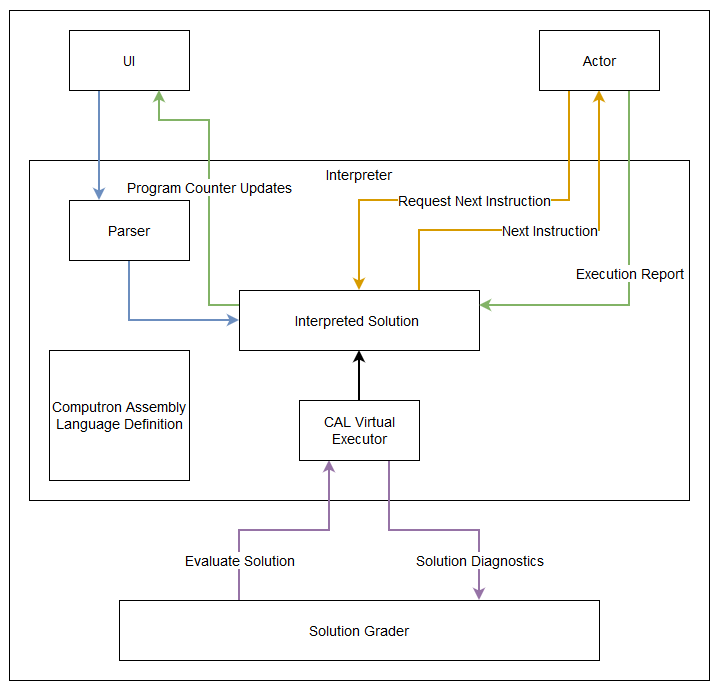
\includegraphics[width=\textwidth]{Diagrams/interpreter_diagram.png}
\end{figure}


\subsubsection{Language}
In order to keep the game accessible to inexperienced users, we developed a simple
pseudo-language to manage the manipulation of the puzzles. Below are the 13 instructions that 
make up the CAL.

\begin{itemize}
 	\item INPUT\\
	The INPUT command instructs Computron to approach the puzzle's Input Box and 
	retrieve the next value. If Computron is currently holding a value, he will discard it. 
	If the Input Box is empty, Computron will retrieve and hold a NULL value.
	\item OUTPUT\\
	The OUTPUT command instructs Computron to approach the puzzle's Output Box 
	and deposit his current value. If Computron is not holding anything, this instruction 
	will be considered invalid and raise a runtime error. Otherwise Computron will deposit 
	the value in the output box.
	\item JUMP\\
	The plain JUMP command instructs the interpreter to unconditionally move the program 
	counter to a new line in the player's solution. This instruction has no effect on Computron.
	\item JUMP IF NULL\\
	The JUMP IF NULL is a conditional jump instruction, which is only activated if the Actor
	 is not holding any value. This instruction is often used to break out of loops.
	\item JUMP IF LESS [X]\\
	The JUMP IF LESS [X] is a conditional jump instruction, which is only activated if the 
	value the Actor is holding is less than the value stored in player-specified memory card X. If 
	memory card X is empty, this instruction will be considered invalid and raise a runtime error.
	\item JUMP IF GREATER [X]\\
	The JUMP IF GREATER [X] is a conditional jump instruction, which is only activated if 
	the value the Actor is holding is greater than the value stored in player-specified memory card 
	X. If memory card X is empty, this instruction will be considered invalid and raise a runtime error.
	\item JUMP IF EQUAL [X]\\
	The JUMP IF EQUAL [X] is a conditional jump instruction, which is only activated if 
	the value the Actor is holding is equal to the value stored in player-specified memory card 
	X. If memory card X is empty, this instruction will be considered invalid and raise a runtime error.
	\item MOVETO [X]\\
	The MOVETO [X] command instructs Computron to move the value currently being 
	held into the player-specified memory card X. If Computron's hands are currently empty, this 
	instruction will be considered invalid and raise a runtime error. If there is a value currently in 
	the memory card, it will be overwritten.
	\item MOVEFROM [X]\\
	The MOVEFROM [X] command instructs Computron to remove the value currently being 
	stored in the player-specified memory card X. If the memory card is empty, Computron will retrieve 
	and hold a NULL value. If Computron is currently holding a value, it will be overwritten.
	\item COPYTO [X]\\
	The COPYTO [X] command instructs Computron to move the value currently being held 
	into the player-specified memory card X. Computron will retain a copy of the number. If 
	Computron's hands are currently empty, this instruction will be considered invalid and raise a 
	runtime error. If there is a value currently in the memory card, it will be overwritten.
	\item COPYFROM [X]\\
	The COPYFROM [X] command instructs Computron to retrieve a copy of the value currently 
	being stored in in the player-specified memory card X. If the memory card is empty, Computron will 
	retrieve and hold a NULL value. If Computron is currently holding a value, it will be overwritten.
	\item ADD [X]\\
	The ADD [X] command instructs Computron to add the value stored in player-specified 
	memory card X to the value currently held. If either Computron's hands or memory card X are empty, this 
	instruction will be considered invalid and raise a runtime error. Otherwise, Computron will 
	perform the addition and overwrite his current value.\\
	\item SUBTRACT [X]\\
	The SUBTRACT [X] command instructs Computron to subtract the value stored in 
	player-specified memory card X from the value currently held. If either Computron's hands or 
	memory card X are empty, this instruction will be considered invalid and raise a runtime error. 
	Otherwise, Computron will perform the subtraction and overwrite his current value.
\end{itemize}

\subsubsection{Program Counter}
To facilitate proper simulation of the player's solution, the interpreter will need to maintain 
a program counter that iterates and jumps through the player's code appropriately. To 
ensure that these updates happen correctly, the Interpreter will need to rely on reports 
from the Actor that state the validity of instructions and the result of conditional expressions.
Updates to the program counter are forwarded to the Puzzle's UI system to maintain a 
visual representation of the program counter while the solution executes.

\subsubsection{UI Interface}
In addition to updating the program counter, the Interpreter is closely tied to the Puzzle UI's primary
control panel. The Start, Step, and Halt buttons all tie directly to the Interpreter's control interface.
Figure \ref{fig:interpreter_UI_interface} illustrates the nature of these interactions.

\begin{figure}[!htb]
	\caption{Interpreter/UI Interface Overview}
	\label{fig:interpreter_UI_interface}
	\centering
	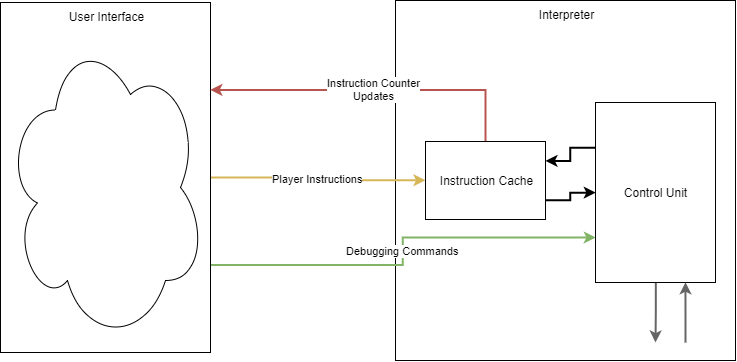
\includegraphics[width=\textwidth]{Diagrams/Interpreter_UI_Interface.png}
\end{figure}

\subsubsection{Actor Interface}
The Interpreter's Actor interface is responsible for making instructions available to the 
Actor on demand. In order to ensure the program counter is updated properly, the 
Interpreter and Actor engage in a three part handshake, shown in 
\ref{fig:interpreter_Actor_interface}.\\

\begin{figure}[!hb]
    \caption{Interpreter/UI Interface Overview}
    \label{fig:interpreter_Actor_interface}
    \centering
    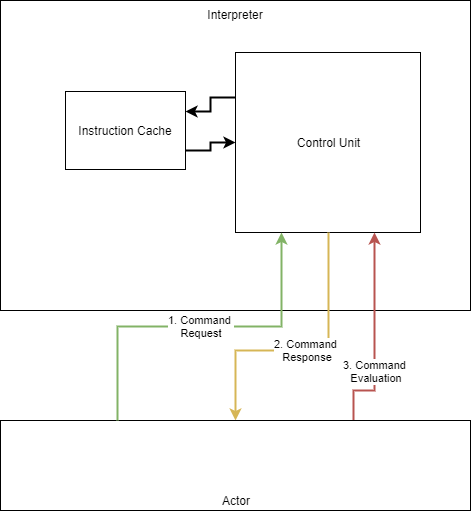
\includegraphics[width=\textwidth]{Diagrams/Interpreter_Actor_Interface.png}
\end{figure}

\newpage
The stages of the handshake are:
\begin{enumerate}
	\item Command Request\\
	The first step of the Actor control exchange is the Command Request. The Actor 
	will issue a Command Request to the Interpreter when the next player instruction is needed.
	\item Command Response\\
	The second step of the exchange is the Command Response. This response will be a 
	data structure for the actor to parse, including the next instruction's opcode and argument.
	\item Command Evaluation\\
	The last step of the exchange is the Command Evaluation. This stage is the Actor's chance 
	to report runtime errors to the Interpreter if the instruction is deemed invalid and report 
	the result of a conditional expression if the instruction included one. 
\end{enumerate}

\subsubsection{CAL Virtual Machine}
The Actor's implementation of the CAL is tightly coupled to the physical state of the puzzle. In addition,
it performs many non-executing tasks to visualize the language. These conditions made the unsuitable for 
conducting performance and correctness evaluations. To support those functions of solution grading the Interpreter
manages a Computron Assembly Language Virtual Machine (CALVM) object. The CALVM allows the interpreter to simulate
player solutions rapidly, and inspect runtime data like error states and cycle count easily. 